\chapter{Solving Equations}


\begin{quote}

%If $A$ is success in life, then $A = x + y + z$. Work is $x$; $y$ is
%play; and $z$ is keeping your mouth shut.
Politics is for the moment. An equation is for eternity.

\hfill---Albert Einstein
\end{quote}


\begin{teachingnote}
In this section, we are developing the idea that numbers are solutions
to equations. Negative integers arise out of simple linear equations,
as do rationals. However, these are not enough to solve all polynomial
equations, and hence we need a ``larger'' number system.
\end{teachingnote}


\section{Time to get Real}

Remember the definition of a \textit{root} of a polynomial:

\begin{definition} A \textbf{root}\index{root} of a polynomial 
\[
a_nx^n + a_{n-1}x^{n-1} + \dots + a_1 x + a_0
\]
is a number $\alpha$ where
\[
a_n\alpha^n + a_{n-1}\alpha^{n-1} + \dots + a_1 \alpha + a_0 = 0.
\]
\end{definition}


OK---let's go! We know what integers are right? We know what rational
numbers are right?

\begin{question}
Remind me, what is $\Z$? What is $\Q$? What is the relationship between
these two sets of numbers?
\end{question}
While I do want \textbf{you} to think about this, I also want to tell
you my answer: $\Q$ is the set of solutions to linear polynomial
equations with coefficients in $\Z$.

\begin{question}
What-with-the-who-in-the-where-now?
\end{question}
\QM

Are these all the numbers we need? Well, let's see. Consider the
innocent equation:
\[
x^2 -2 = 0
\]

\begin{question}
Could $x^2 -2$ have rational roots?
\end{question}

\begin{teachingnote}
Here we essentially run through the proof of the rational roots test.
\end{teachingnote}

Stand back---I'll handle this. Remember, a root of $x^2-2$ is a number
that solves the equation
\[
x^2-2 = 0.
\]
So suppose that there are integers $a$ and $b$ where $a/b$ is a root
of $x^2 -2$ where $a$ and $b$ have no common factors. Then
\[
\left(\frac{a}{b}\right)^2 -2 = 0.
\]
So
\[
a^2 - 2b^2 = 0 \qquad\text{thus}\qquad a^2 = 2b^2.
\]
But $a$ and $b$ have no common factors---so by the Unique
Factorization Theorem \index{Unique Factorization Theorem}for the
integers, $b^2 = 1$. If you find this step confusing, check
  out Problem \ref{P:helper} in Section \ref{S:EA}. This tells us that
$a^2 = 2$ and that $a$ is an integer---impossible! So $x^2-2$ cannot
have rational roots.

Hmmm but now consider the plot of $y= x^2-2$:
\[
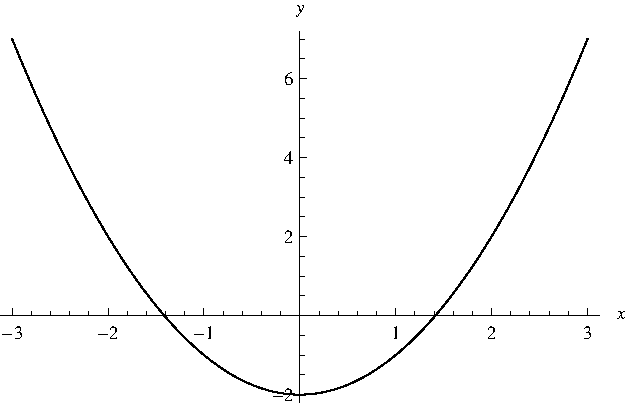
\includegraphics[width=3in]{../graphics/quad2Plot.pdf}
\]
The polynomial $x^2-2$ clearly has two roots! But we showed above that
neither of them are rational---this means that there must be numbers
that cannot be expressed as fractions of integers! In particular, this
means:\index{sqrt2@$\sqrt{2}$} 
\begin{center}
\textbf{The square-root of $\boldsymbol{2}$ is not rational!}
\end{center}
Wow! But it still can be written as a decimal
\[
\sqrt{2} = 1.4142135623\dots \index{sqrt2@$\sqrt{2}$}
\]
as the square-root of $2$ is a \textit{real number}.

\begin{definition}\index{R@$\R$}\index{real numbers} 
A \textbf{real number} is a number with a (possibly
infinite) decimal representation.  We use the symbol $\R$ to denote
the real numbers.
\end{definition}

For example:
\[
-1.000\dots \qquad 2.718281828459045\dots \qquad 3.333\dots \qquad 0.000\dots
\]
are all real numbers.

\begin{question} 
Another description of real numbers is that they are the numbers that
can be approximated by rational numbers. Why does this follow from the
definition above?
\end{question}
\QM

Famous examples of real numbers that are not rational are
\[\index{e@$e$}\index{pi@$\pi$}
\pi = 3.14159265358\dots\qquad \text{and}\qquad e = 2.718281828459045\dots
\]

\begin{question}
If $a$ and $b$ are integers with $b \ne 0$, what can you say about the
decimal representation of $a/b$? What can you say about the decimal
representation of an irrational number?
\end{question}
\QM


\begin{teachingnote}
This is an opportunity to revisit the ideas from activities~\ref{A:DecNotNice} and~\ref{A:Shampoo}. 
\end{teachingnote}


\newpage

\begin{problems}
\begin{enumerate}
\item Describe the set of real numbers. Give some relevant and
  revealing examples/nonexamples.
\item Explain what would happen if we ``declared'' the value of $\pi$
  to be $3$? What about if we declared it to have the value of $3.14$?
\item Explain why $x^2 - x - 1$ has no rational roots. 
\item Explain why $\sqrt{7}$ is irrational.
\item Explain why $\sqrt[3]{5}$ is irrational.
\item Explain why $\sqrt[5]{27}$ is irrational.
\item Explain why if $n$ is an integer and $\sqrt{n}$ is not an
  integer, then $n$ is irrational.
\item Consider the following numbers:
\[
\frac{1}{47} \qquad\text{and}\qquad \frac{1}{78125}
\]
For each, determine whether the decimal representation terminates or
repeates, \textbf{without} actually computing the decimal
representation. Explain your reasoning. If the decimal repeats,
indicate and explain what the maximum possible number of digits in the
repeating pattern is.
\item Solve $x^5 - 31x^4 +310x^3 -1240 x^2 + 1984x-1024= 0$. Interlace
  an explanation with your work. Hint: Use reasoning from this section
  to find rational roots.
\item Solve $x^5 - 28x^4 +288x^3 - 1358 x^2 + 2927 x -2310 =
  0$. Interlace an explanation with your work. Hint: Use reasoning
  from this section to find rational roots.
\item Knowing that $\pi$ is irrational, explain why $101\cdot\pi$ is
  irrational.
\item Knowing that $\pi$ is irrational, explain why $\pi + 101$ is
  irrational.
\item Knowing that $\pi$ is irrational, explain why $77.2835\cdot\pi$ is
  irrational.
\item Knowing that $\pi$ is irrational, explain why $\pi + 77.2835$ is
  irrational.
\item Suppose we knew that $\alpha^2$ was irrational. Could we
  conclude that $\alpha$ is also irrational? Explain your reasoning.
\item Is $((\sqrt{2})^{\sqrt{2}})^{\sqrt{2}}$ rational or irrational?
  Explain your reasoning.
\item In the discussion above, we give an argument showing that
  $\sqrt{2}$ is irrational. What happens if you try to use the exact
  same argument to try and show that $\sqrt{9}$ is irrational? Explain
  your reasoning.
\item For each of the following statements, indicate whether the expression
is a ``rational number,'' an ``irrational number,'' or whether it could be
either. Note, in parts (d)--(f) assume that neither numbers are zero.
\begin{enumerate}
\item $\text{rational}+ \text{rational} = ?$
\item $\text{rational}+ \text{irrational} = ?$
\item $\text{irrational}+ \text{irrational} = ?$

\item $\text{rational}\cdot \text{rational} = ?$
\item $\text{rational}\cdot \text{irrational} = ?$
\item $\text{irrational}\cdot \text{irrational} = ?$
\end{enumerate}
Give careful explanations for parts (a), (e), and (f).
\end{enumerate}
\end{problems}
\newpage




\section{Polynomial Equations}


\begin{activitynote}
Activity~\ref{A:HAlgebra} is a good warm-up to this section.  % Hieroglyphical Algebra
\end{activitynote}

Solving equations is one of the fundamental activities in mathematics.
We're going to separate our equations into sets:
\begin{enumerate}
\item Linear Equations---polynomial equations of degree $1$.
\item Quadratic Equations---polynomial equations of degree $2$.
\item Cubic  Equations---polynomial equations of degree $3$.
\item Quartic Equations---polynomial equations of degree $4$.
\item Quintic Equations---polynomial equations of degree $5$.
\end{enumerate}
We'll stop right there, for now\dots


\subsection{Linear Equations}

The simplest polynomials (besides constant polynomials) are linear
polynomials. Solving equations of the form
\[
ax + b = 0
\]
poses no difficulty, we can write out the solution easily as
\[
x = -b/a.
\]



\subsection{Quadratic Equations}\index{completing the square}

Finding roots of quadratic polynomials is a bit more complex. We want
to find $x$ such that
\[
ax^2 + bx + c = 0.
\]
I know you already know how to do this. However, pretend for a moment
that you don't. This would be a really hard problem. We have evidence
that it took humans around 1000 years to solve this problem in
generality, the first general solution appearing in Babylon and China
around 2500 years ago. With this in mind, I think this topic warrants
some attention. If you want to solve $ax^2 + bx + c = 0$, a good place
to start would be with an easier problem. Let's make $a=1$ and try to
solve
\[
x^2 + b x = c
\]
Geometrically, you could visualize this as an $x \times x$ square
along with a $b\times x$ rectangle. Make a blob for $c$ on the other side. 

\begin{question} What would a picture of this look like?
\end{question}
\QM

\begin{question} What is the total area of the shapes in your picture?
\end{question}
\QM

Take your $b\times x$ rectangle and divide it into two
$(b/2)\times x$ rectangles.

\begin{question} What would a picture of this look like?
\end{question}
\QM

\begin{question} What is the total area of the shapes in your picture?
\end{question}
\QM

Now take both of your $(b/2)\times x$ rectangles and snuggie them
next to your $x\times x$ square on adjacent sides. You should now have
what looks like an $(x + \frac{b}{2}) \times (x +
\frac{b}{2})$ square with a corner cut out of it.


\begin{question} What would a picture of this look like?
\end{question}
\QM

\begin{question} What is the total area of the shapes in your picture?
\end{question}
\QM

Finally, your big $(x + \frac{b}{2}) \times (x + \frac{b}{2})$ has a
piece missing, a $(b/2) \times (b/2)$ square, right? So if you add
that piece in on both sides, the area of both sides of your picture
had better be $c + (b/2)^2$. From your picture you will find that:
\[
\left(x + \frac{b}{2}\right)^2 = c + \left(\frac{b}{2}\right)^2
\]

\begin{question} 
Can you find $x$ at this point?
\end{question}
\QM

\begin{question}
Explain how to solve $ax^2 + bx + c = 0$.
\end{question}
\QM




\begin{activitynote}
Activities~\ref{A:otherSide},~\ref{A:vertex}, and~\ref{A:leastSquares},
complement this section well.
% The Other Side--Solving Equations, Maximums and Minimums, Least Squares Approximation
\end{activitynote}

\begin{activitynote}
Activity~\ref{A:otherCurves} could be done here too.  % It Takes All Kinds
\end{activitynote}

\subsection{Cubic Equations}

While the quadratic formula was discovered around 2500 years ago,
cubic equations proved to be a tougher nut to crack. A general
solution to a cubic equation was not found until the 1500's. At the
time mathematicians were a secretive and competitive bunch. Someone
would solve a particular cubic equation, then challenge another
mathematician to a sort of ``mathematical duel.'' Each mathematician
would give the other a list of problems to solve by a given date. The
one who solved the most problems was the winner and glory
everlasting\footnote{This might be a slight exaggeration.}  was
theirs. One of the greatest duelists was Niccol\`{o} Fontana Tartaglia
(pronounced \textit{Tar-tah-lee-ya}). Why was he so great? He
developed a general method for solving cubic equations! However,
neither was he alone in this discovery nor was he the first. As
sometimes happens, the method was discovered some years earlier by
another mathematician, Scipione del Ferro. However, due to the secrecy
and competitiveness, very few people knew of Ferro's method. Since these
discoveries were independent, we'll call the method the
\textit{Ferro-Tartaglia method}.

We'll show you the Ferro-Tartaglia method\index{Ferro-Tartaglia
  method} for finding at least one root of a cubic of the form:
\[
x^3+ px + q
\]
We'll illustrate with a specific example---you'll have to generalize
yourself! Take
\[
x^3 +3x - 2  = 0
\]
\paragraph{Step 1} Replace $x$ with $u+v$. 
\begin{align*}
(u+v)^3 + 3(u+v) - 2  &= u^3 + 3u^2v + 3uv^2 + v^3 + 3(u+v) -2 \\
&= u^3 + v^3 + 3uv(u+v) + 3(u+v) - 2\\
&= u^3 + v^3 - 2 + (3uv+3)(u+v).
\end{align*}
\paragraph{Step 2} 
Set $uv$ so that all of the terms are eliminated except for $u^3$,
$v^3$, and constant terms.  

Since we want 
\[
3uv + 3 = 0
\]
we'll set $uv = -1$ and so 
\[
u^3 + v^3 -2 = 0.
\]
Since $uv = -1$, we see that $v = -1/u$ so
\[
u^3 + \left(\frac{-1}{u}\right)^3  -2 = u^3 - \frac{1}{u^3} - 2= 0.
\]
\paragraph{Step 3} 
Clear denominators and use the quadratic formula.
\[
u^3 - \frac{1}{u^3} -2 = 0 \qquad \Leftrightarrow \qquad u^6 - 2 u^3 -1 = 0
\]
But now we may set $y = u^3$ and so we have
\[
y^2 - 2y -1 = 0
\]
and by the quadratic formula
\[
y = \frac{2 \pm \sqrt{4 + 4}}{2} = 1 \pm \sqrt{2}.
\]
Putting this all together we find:
\begin{align*}
y &= 1 \pm \sqrt{2} \\
u &= \sqrt[3]{1 \pm \sqrt{2}}\\
v &= \frac{-1}{\sqrt[3]{1 \pm \sqrt{2}}}
\end{align*}
and finally (drum-roll please):
\[
x = \sqrt[3]{1 + \sqrt{2}} - \frac{1}{\sqrt[3]{1 + \sqrt{2}}} \qquad\text{and}\qquad x = \sqrt[3]{1 - \sqrt{2}} - \frac{1}{\sqrt[3]{1 - \sqrt{2}}}
\]

\begin{question} How many solutions are we supposed to have in total?
\end{question}
\QM


\begin{question} How do we do this procedure for other equations of the form
\[
x^3 + px + q = 0?
\]
\end{question}
\QM



\subsection{Quartics, Quintics, and Beyond}

While the Ferro-Tartaglia method may seem like it only solves the
special case of $x^3 + px +q = 0$, it is in fact a ``wolf in sheep's
clothing''\index{wolf in sheep's clothing} and is the key to giving a
formula for solving any cubic equation
\[
ax^3 + bx^2 + cx +d = 0.
\]
The formula for solutions of the cubic equation is quite complex---we
will spare you the details. Despite the fact that the key step of the
formula is the Ferro-Tartaglia method, it is usually called
\textit{Cardano's formula}\index{Cardano's formula} because Cardano
was the first to publish this method.

It was wondered if there were formulas for solutions to polynomial
equations of arbitrary degree. When we say formulas, we mean formulas
involving the coefficients of the polynomials and the symbols:
\[
+\quad -\quad \cdot\quad \div \quad \sqrt{\hspace{1em}}
\]
Cardano's student Ferrari, (who incidentally went to the University of
Bologna) soon found the quartic formula, though it is too monstrous to
write down in these notes. The search for the quintic equation
began. Things started getting very difficult. The old tricks didn't
work, and it wasn't until nearly 300 years later that this problem was
settled.

\begin{question} 
Who was Niels Abel? Who was \'{E}variste
Galois?\index{Abel}\index{Galois}
\end{question}
\QM

Abel and Galois (pronounced \textit{Gal-wah}), independently prove
that there is no general formula (using only the symbols above) for
polynomial equations of degree $5$ or higher. It is an amazing result
and is only seen by students in advanced undergraduate or beginning
graduated courses in pure mathematics. Nevertheless, in our studies we
will not completely shy away from such demons. Read on!






\newpage

\begin{problems}
\begin{enumerate}
\item Draw a rough timeline showing: The point when we realized we
  were interested in quadratic equations, the discovery of the
  quadratic formula, the discovery of the cubic formula, the discovery
  of the quartic formula, and the work of Abel and Galois proving the
  impossibility of a general formula for polynomial equations of
  degree 5 or higher.
\item Given a polynomial, explain the connection between
  \textit{linear factors} and \textit{roots}. Are they the same thing
  or are they different things?
\item In ancient and Medieval times the discussion of quadratic
  equations was often broken into three cases:
\begin{enumerate}
\item $x^2 + bx = c$
\item $x^2 = bx + c$
\item $x^2 + c = bx$
\end{enumerate}
where $b$ and $c$ are positive numbers. Create real-world word
problems involving length and area for each case above.
\item In ancient and Medieval times the discussion of quadratic
  equations was often broken into three cases:
\begin{enumerate}
\item $x^2 + bx = c$
\item $x^2 = bx + c$
\item $x^2 + c = bx$
\end{enumerate}
where $b$ and $c$ are positive numbers.  Is this a complete list of
cases? If not, what is missing and why is it (are they)
missing? Explain your reasoning.
\item Describe what happens geometrically when you complete the square
  of a quadratic equation of the form $x^2 + bx = c$ when $b$ and $c$
  are positive. Explain your reasoning.
\item Jim, Lydia, and Isabel are visiting China. Unfortunately they are
  stuck in a seemingly infinite traffic jam. The cars are moving at a
  very slow (but constant) rate. Jim and Lydia are 25 miles behind
  Isabel. Jim wants to send a sandwich to Isabel. So he hops on his
  motorcycle and rides through traffic to Isabel, gives her the
  sandwich, and rides back to Lydia at a constant speed. When he
  returns to Lydia, she has moved all the way to where Isabel was when
  Jim started. In total, how far did Jim travel on his motorcycle?
\begin{enumerate}
\item Before any computations are done, use common sense to guess the
  solution to this problem.
\item Try to get a feel for this problem by choosing numbers for the
  unknowns and doing some calculations. What do these calculations say
  about your guess?
\item Use algebra to solve the problem.
\end{enumerate}
\item Must a quadratic polynomial always have a real root? Explain
  your reasoning.
\item Must a cubic polynomial always have a real root? Explain your
  reasoning.
\item Must a quartic polynomial always have a real root? Explain your
  reasoning.
\item Must a quintic polynomial always have a real root? Explain your
  reasoning.
\item Derive the quadratic formula. Explain your reasoning.
\item Solve $x^2 + 3x -2 = 0$. Interlace an explanation with your work.
\item Find two solutions to $x^4 + 3x^2 -2 = 0$. Interlace an
  explanation with your work.
\item Find two solutions to $x^6 + 3x^3 -2 = 0$. Interlace an
  explanation with your work.
\item Find two solutions to $x^{10} + 3x^5 -2 = 0$. Interlace an
  explanation with your work.
\item Find two solutions to $3x^{14} - 2x^7 + 6 = 0$. Interlace an
  explanation with your work.
\item Find two solutions to $-4x^{22} + 13x^{11} + 1 = 0$. Interlace
  an explanation with your work.
\item Give a general formula for finding two solutions to equations of
  the form: $ax^{2n} + bx^{n} + c = 0$ where $n$ is an
  integer. Interlace an explanation with your work.
\item Use the Ferro-Tartaglia method to find a solution to $x^3+x+1 =
  0$. Interlace an explanation with your work.
\item Use the Ferro-Tartaglia method to find a solution to $x^3-x-1 =
  0$. Interlace an explanation with your work.
\item Use the Ferro-Tartaglia method to find a solution to $x^3+3x-4 =
  0$. Interlace an explanation with your work.
\item Use the Ferro-Tartaglia method to find a solution to $x^3+2x-3 =
  0$. Interlace an explanation with your work.
\item Use the Ferro-Tartaglia method to find a solution to $x^3+6x-20 =
  0$. Interlace an explanation with your work.
\item Find at least two solutions to $x^4-x^3-3x^2+2x+1 =0$. Hint: Can
  you ``guess'' a solution to get you started?  Interlace an
  explanation with your work.
\item Explain what Abel and Galois proved to be impossible.
\end{enumerate}
\end{problems}





\section{Me, Myself, and a Complex Number}

\begin{activitynote}
Activity~\ref{A:sketchRoots} complements this section well.  % Sketching Roots
\end{activitynote}


We'll start with the definition:

\begin{definition} 
A \textbf{complex number}\index{C@$\C$}\index{complex!numbers} is a
number of the form
\[
x + yi
\]
where $x$ and $y$ are real numbers and $i$ is the square-root of
negative one. We use the symbol $\C$ to denote the complex numbers.
\end{definition}

What's that I hear? Yells of protest telling me that no such number
exists? Well if it makes you feel any better, people denied the
existence of such numbers for a long time. It wasn't until the
$1800$'s until people finally changed their minds. Let's talk about
some ideas that helped. Consider the plot of $y = x^3-6x+1$:
\[
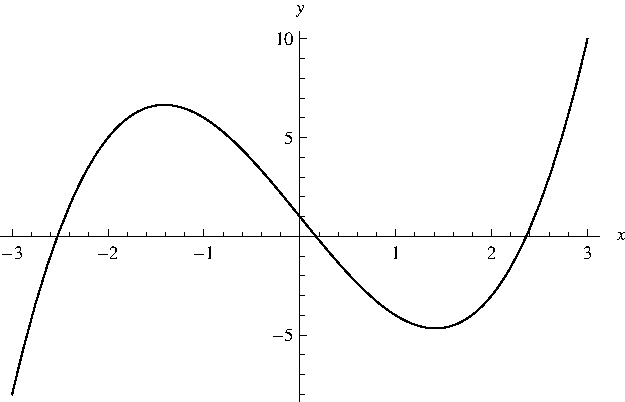
\includegraphics[width=3in]{../graphics/cubicPlot.pdf}
\]
If you use the Ferro-Tartaglia method to find at least one solution to
this cubic, then you find the following root:
\[
\sqrt[3]{\frac{-1+\sqrt{-31}}{2}} + \frac{2}{\sqrt[3]{\frac{1}{2}(-1+\sqrt{-31})}}
\]
This root looks like a complex number, since $\sqrt{-31}$ pops up
twice.  This might seem a bit redundant, but we should point out that
$\sqrt{-31}$ is a complex number since it can be expressed as:
\[
0 + \left(\sqrt{31}\right) i
\]
Even though our root has complex numbers in it, we know that it is
real from the picture!  Moral: If you want to give exact solutions to
equations, then you'd better work with complex numbers, even if the
roots are real!

\begin{teachingnote}
Here we are not ready to try to simplify the large expression
above. We are leaving this as a mystery for a future course.
\end{teachingnote}


\begin{question} If $u+vi$ is a nonzero complex number, is 
\[
\frac{1}{u+vi}
\]
a complex number too?
\end{question}

You betcha! Let's do it. The first thing you must do is multiply the
numerator and denominator by the complex conjugate of the denominator:
\[
\frac{1}{u+vi} = \frac{1}{u+vi} \cdot \frac{u-vi}{u-vi} =\frac{u-vi}{u^2 + v^2}
\]
Now break up your fraction into two fractions:
\[
\frac{u-vi}{u^2 + v^2} = \frac{u}{u^2 + v^2} + \frac{-v}{u^2+v^2}i
\]
Ah! Since $u$ and $v$ are real numbers, so are
\[
x = \frac{u}{u^2 + v^2} \qquad \text{and}\qquad y = \frac{-v}{u^2+v^2}
\]
Hence 
\[
\frac{1}{u+vi} = x + yi
\]
and is definitely a complex number.

The real importance of the complex numbers came from
Gauss,\index{Gauss} with the Fundamental Theorem of Algebra:

\begin{theorem}[Fundamental Theorem of Algebra]
\index{Fundamental Theorem!of Algebra} Every polynomial of the form
\[
 a_n x^n + a_{n-1} x^{n-1} + \dots + a_1 x + a_0
\]
where the $a_i$'s are complex numbers has exactly $n$ (possibly
repeated) complex roots.
\end{theorem}

Said a different way, the Fundamental Theorem of Algebra says that
every polynomial with complex coefficients
\[
a_n x^n + a_{n-1} x^{n-1} + \dots + a_1 x + a_0
\]
can be factored as 
\[
a_n\cdot (x-r_1)(x-r_2) \cdots (x-r_n)
\]
where each $r_i$ is a complex number.

\begin{question} 
How many complex roots does $x^3-1$ have? What are they?
\end{question}
\QM

\begin{teachingnote}
This problem should definitely be addressed. Again, we find an
obvious root, $x=1$ and use the division theorem.
\end{teachingnote}



\subsection{The Complex Plane}


\begin{activitynote}
Activities~\ref{A:complexAddition} and~\ref{A:complexMultiplication}
complement this section well.
\end{activitynote}

Complex numbers have a strong connection to geometry, we see this with
the \textit{complex plane}:

\begin{definition}
The \textbf{complex plane}\index{complex!plane} is obtained when one
plots the complex number $x + yi$ as the point $(x,y)$. When
considering the complex plane, the horizontal axis is called the
\textbf{real axis} and the vertical axis is called the
\textbf{imaginary axis}.
\end{definition}

Here is a grid. Draw the real and imaginary axes and plot the complex
numbers:
\[
3 \qquad -5i \qquad 4+6i \qquad -3+5i \qquad -6 -i \qquad 6-6i
\]
\[

\includegraphics{../graphics/complexPlane.pdf}
\]
Be sure to label your plot.


\begin{question} 
Geometrically speaking, what does it mean to ``add'' complex numbers?
\end{question}
\QM

\begin{question} 
Geometrically speaking, what does it mean to ``multiply'' complex numbers?
\end{question}
\QM

\begin{activitynote}
Activity \ref{A:deg2Ext} is worth considering here.
\end{activitynote}


\newpage

\begin{problems}
\begin{enumerate}
\item What is a real number?
\item What is a complex number?
\item Solve $x^3-6x+5 = 0$ two different ways. First, try to find an
  ``obvious'' root, call it $r$. Then divide your polynomial by
  $(x-r)$ and find the remaining roots. Second, use the
  Ferro-Tartaglia method to find (at least) one solution. Compare your
  answers. What do you notice---explain your reasoning.
\item Solve $x^3-6x+4 = 0$ two different ways. First, try to find an
  ``obvious'' root, call it $r$. Then divide your polynomial by
  $(x-r)$ and find the remaining roots. Second, use the
  Ferro-Tartaglia method to find (at least) one solution. Compare your
  answers. What do you notice---explain your reasoning.
\item Solve $x^3-2x-1 = 0$ two different ways. First, try to find an
  ``obvious'' root, call it $r$. Then divide your polynomial by
  $(x-r)$ and find the remaining roots. Second, use the
  Ferro-Tartaglia method to find (at least) one solution. Compare your
  answers. What do you notice---explain your reasoning.  Interlace an
  explanation with your work.
\item Solve $x^3-12x-8 = 0$ two different ways. First, try to find an
  ``obvious'' root, call it $r$. Then divide your polynomial by
  $(x-r)$ and find the remaining roots. Second, use the
  Ferro-Tartaglia method to find (at least) one solution. Compare your
  answers. What do you notice---explain your reasoning.  Interlace an
  explanation with your work.
\item Solve $x^3-3x^2+5x-3 = 0$. Hint: Can you ``guess'' a solution to
  get you started?  Interlace an explanation with your work.
\item Solve $x^3+4x^2-7x+2 = 0$. Hint: Can you ``guess'' a solution to
  get you started?  Interlace an explanation with your work.
\item Draw a Venn diagram showing the relationship between $\Z$, $\Q$,
  $\R$, and $\C$. Include relevant examples of numbers belonging to
  each set.
\item Explain why the following ``joke'' is ``funny:'' \textit{The
  number you have dialed is imaginary. Please rotate your phone by 90
  degrees and try again.}
\item Explain why every real number is a complex number.
\item Explain why $\sqrt{-2}$ is a complex number. 
\item Is $\sqrt[3]{-2}$ a complex number? Explain your reasoning.
\item Explain why $\sqrt[10]{-5}$ is a complex number.
\item Explain why if $x+yi$ and $u+vi$ are complex numbers, then 
\[
(x+yi) +(u+vi)
\]
is a complex number.
\item Explain why if $x+yi$ and $u+vi$ are complex numbers, then 
\[
(x+yi)(u+vi)
\]
is a complex number.
\item Given a complex number $z = x + yi$, the \textbf{complex conjugate} of\index{complex!conjugate}
  $z$ is $x-yi$, we denote this as $\bar{z}$. Let $w = u+vi$ be
  another complex number.
\begin{enumerate}
\item Explain why $\bar{z}+\bar{w} = \bar{z+w}$.
\item Explain why $\bar{z}\cdot\bar{w} = \bar{z\cdot w}$.
\end{enumerate}
\item Explain why if $u+vi$ is a complex number, then
\[
\frac{1}{u+vi}
\]
is a complex number.
\item Compute the following, expressing your answer in the form
  $x + yi$:
\begin{enumerate}
\item $(1 + 2i)+ (1+7i)$
\item $(1 + 2i)\cdot (1+7i)$
\item $(1 + 2i)/(1+7i)$
\end{enumerate}
Explain your reasoning.
\item I'm going to show you something, see if you can see a connection to geometry:
\begin{enumerate}
\item Let $z = 3 + 4i$. Compute $\sqrt{z\cdot \bar{z}}$. 
\item Let $z = 6 + 8i$. Compute $\sqrt{z\cdot \bar{z}}$. 
\item Let $z = 5 + 12i$. Compute $\sqrt{z\cdot \bar{z}}$. 
\end{enumerate}
What do you notice?
\item\label{P:sqrti} Express $\sqrt{i}$ in the form $a + bi$. Hint: Solve the
  equation $z^2 = i$.
\item Factor the polynomial $3x^2 + 5x + 10$ over the complex
  numbers. Explain your reasoning.
\item Factor the polynomial $x^3-1$ over the complex numbers. Explain
  your reasoning.
\item Factor the polynomial $x^4-1$ over the complex numbers. Explain
  your reasoning.
\item Factor the polynomial $x^4+1$ over the complex numbers. Explain
  your reasoning. Hint: Factor as the difference of two squares and use Problem~\ref{P:sqrti}. 
\item Factor the polynomial $x^4+4$ over the complex numbers. Can it
  be factored into polynomials with real coefficients of lower degree?
  Explain your reasoning.
\item Plot all complex numbers $z$ in the complex plane such that
  $z\cdot \bar{z} =1$. Explain your reasoning.
\item\label{P:taylor} Suppose I told you that:
\begin{align*}
\sin(x) &= x - \frac{x^3}{3!} + \frac{x^5}{5!} - \frac{x^7}{7!} + \dots + \frac{(-1)^n x^{2n+1}}{(2n+1)!} + \cdots \\
\cos(x) &= 1 - \frac{x^2}{2!} + \frac{x^4}{4!} - \frac{x^6}{6!} + \dots + \frac{(-1)^n x^{2n}}{(2n)!} + \cdots \\
e^x &= 1 + x + \frac{x^2}{2!} + \frac{x^3}{3!} + \frac{x^4}{4!} + \dots + \frac{x^n}{n!} + \cdots 
\end{align*}
Explain why we say:
\[
e^{x\cdot i} = \cos(x) + i \sin(x)
\]
\item This is Euler's famous formula:
\[
e^{\pi \cdot i } + 1 = 0
\]
Use Problem \ref{P:taylor} to explain why it is true.
\item How many complex roots should $x^2 = 1$ have? What are they?
  Plot them in the complex plane.  Explain your reasoning.
\item How many complex roots should $x^3 = 1$ have? What are they?
  Plot them in the complex plane.  Explain your reasoning.
\item How many complex roots should $x^4 = 1$ have? What are they?
  Plot them in the complex plane.  Explain your reasoning.
\item How many complex roots should $x^5 = 1$ have? What are they?
  Plot them in the complex plane.  Explain your reasoning.




\end{enumerate}
\end{problems}
%%
%% Add cube root of unity, w
%% u+v
%% wu + v
%% u + wv
%%


